\section{Simulation}
\label{sec:simulation}

The authors simulate the estimation of the Roy model, a discrete choice model which has intractable likelihood for certain parameter values.

\subsection{The Roy model}
\label{sec:roy}

The Roy model models a set of agents chosing which sector to work in in each of two time periods.
At the start of the game, nature determines the (natural logarithms of the) wages offered to each agent, by the following formulas:
\begin{equation} %fix indicator and make new line
    \text{log} w_{i1s} = \mu_s + \varepsilon_{i1s}
    \text{log} w_{i2s} = \mu_s + \gamma \mathbb{1} {d_{i1} = s} + \varepsilon_{i2s} %fix indicator
\end{equation}
where the noise of the offered wages is distributed as follows:
\begin{equation}
    \left[\begin{array}{l}\varepsilon_{i 11} \\ \varepsilon_{i 12} \\ \varepsilon_{i 21} \\ \varepsilon_{i 22}\end{array}\right] \sim N\left(\left[\begin{array}{l}0 \\ 0 \\ 0 \\ 0\end{array}\right],\left[\begin{array}{cccc}\sigma_1^2 & \rho_s \sigma_1 \sigma_2 & \rho_t \sigma_1^2 & \rho_s \rho_t \sigma_1 \sigma_2 \\ \rho_s \sigma_1 \sigma_2 & \sigma_2^2 & \rho_s \rho_t \sigma_1 \sigma_2 & \rho_t \sigma_2^2 \\ \rho_t \sigma_1^2 & \rho_s \rho_t \sigma_1 \sigma_2 & \sigma_1^2 & \rho_s \sigma_1 \sigma_2 \\ \rho_s \rho_t \sigma_1 \sigma_2 & \rho_t \sigma_2^2 & \rho_s \sigma_1 \sigma_2 & \sigma_2^2\end{array}\right]\right).
\end{equation}

In the first time period, each agent $i$ observes the wages log $w_{i11}$ and log $w_{i12}$ offered to them in the two sectors.
Knowing their own discount factor $\beta$ and the parameters $\gamma_1$ and $\gamma_2$, they solve the dynamic progamming problem
and pick a sector for the first period.
In the second period, they the wages log $w_{i21}$ and log $w_{i12}$ are revealed to them and they pick a sector. %Formula

The researcher observes the realized wages log $w_1$ and log $w_2$ and as well as the corresponding sector choices $d_1, d_2 \in {1, 2}$.
Broadly speaking, the parameters $\mu_1$, $\mu_2$, and to a lesser degree $\gamma_1$ and $\gamma_2$, are location parameters of the distributions of offered wages,
while $\sigma_1$, $\sigma_2$, $\rho_s$ and $\rho_t$ determine the shape and corrrelations (shapes of the joint distributions). %TODO check

Note the selection effects resulting from only realized wages being observed.
In particular, if $\mu_i$ is suffiently below $\mu_j$, sector $i$ will never be picked and $\mu_i$ will not be identified.

If $rho_t = 0$, a likelihood function for observations from the Roy model is available.

\subsection{General simulation structure}
\label{sec:general_simulation_structure}

First, I reproduce parts of the authors' simulation in the scientific Python stack, more precisely, using the packages numpy, scipy, and scikit-learn (\textcite{harris2020array}, \textcite{2020SciPy-NMeth}, and \textcite{scikit-learn}, respectively).
My code is available %TODO %on GitHub? %upon request?
%TODO cite Matlab?

I program another simulation using \texttt{PyTorch} (\cite{Ansel_PyTorch_2_Faster_2024}), a popular and highly developed neural network library for Python.
Among the advantages of Pytorch is that it offers support for training neural networks on GPUs %TODO which has what precise advantages?
Additionally, the library \texttt{GeomLoss} (\cite{feydy2019interpolating}) builds on PyTorch. 
Its \texttt{SampleLoss} function provides the Sinkhorn approximations of the Wasserstein-1 and -2 distances.
It is also optimized for running on GPUs by virtue of being built on \texttt{KeOps} (\cite{KeOps}).
%Besides the Wasserstein loss, I also add several other best practices taken from \cite{athey2021using}.

For my scientific Python code, I use the \texttt{mp} module from Python's standard library to parallelize simulation runs on an HPC cluster (cf. \ref{sec:acknowledgement_of_system_use}).
I generate plots using \texttt{Matplotlib} (\cite{Matplotlib}).

The replication package of \cite{kaji2023adversarial} can be downloaded from the journal website.
It contains the authors' simulation code, written in Matlab. %TODO cite?
As the authors state in the readme file, the simulations for the Roy model are contained in the files \texttt{main\_roy.m} (Figures 6, 7) and \texttt{main\_case.m} (Figures 8, 9, and Table I).
They draw on functions in other files to simulate data and calculate losses.

Both main files share a general structure:
After setting parameters of the simulation itself (e.g. sample sizes, number of simulation runs) and the Roy model, the values of loss functions are calculated along a linear grid and then rendered to created Figures 6 and 8.
The grid describes seven- or eight-dimensional ``cross-hairs'', where one parameters is varied while the others remain fixed at the true value.
Thereafter, real and fake observations are generated and an intial guess in generated.
Then, the the Roy model is estimated using multiple methods, which are implemented as a constrained minimizations.% of a loss function which in turn calculates the discriminators. %TODO write better
The constraints are bounds on the parameters of the Roy model, on which the authors do not futher elaborate, but which are likely added for computational efficiency. %TODO true?
Where necessary, an additional nonlinear constraint enforces that the guesses of the minimizer stay within the support of the Roy model.

\begin{algorithm}
    \caption{Initial guess in main\_roy.m}
    \label{alg:theta0}
    \begin{algorithmic}
        \STATE Input: True parameter vector $\theta$, lower and upper bounds L, U, the support of the Roy model $\mathcal{S}$
        \WHILE{$\theta_{0,p} \notin \mathcal{S}$, for each parameter p of $\theta$ to be estimated:}
            \STATE Sample noise $u_p \sim \mathcal{N}(0, 0.2)$
            \STATE Set $\theta_{0,p} := \theta_p + u_p$
            \STATE Clip $\theta_{0,p} := min(max(\theta_{0,p}, L_p), U_p)$
        \ENDWHILE
    \end{algorithmic}
\end{algorithm}

In \texttt{main\_roy.m}, the authors plot cross-sections of the loss landscapes generated by the Oracle and neural network discriminator as well as the loss implied by MLE. %TODO wording
Then, they generate the intial guess $\theta_0$ using \ref{alg:theta0}.
Following simple maximum likelihood estimation with $\theta_0$ as an intial value, they perform adversarial estimation with:
\begin{itemize}
    \item the Oracle discriminator, using the result of MLE as intial value
    \item the Logistic discriminator, using the result of the previous step as initial value
    \item the neural network discriminator, again using the result of the Oracle step as intial value
\end{itemize} 
They also estimate the Roy model using Indirect Infernce and optimally-weighted SMM, but don't use the results.

\texttt{Main\_case.m} simulates untractable likelihood case
Therefore, an initial guess $\theta_0$ is drawn similarly algorithm \ref{alg:theta0}, but the first draw is used.
Logistic regression is then perfomed using $\theta_0$ as an intial value, and the result used to intialized adversarial estimation. %TODO loss 1 and to
Again, loss-curves for the neural network and logistic discriminator are plotted, including for $\rho_t$.
To study the properties of the adversarial estimators, \textcite{kaji2023adversarial} then perform the bootstrap, sampling with replacement from the noise and the true observations independently.
They perform estimation with the logistic discriminator using the previous logistic estimate as initial value.
The result of this serves as initial value for estimation with the neural network discriminator, as well as for the Indirect Inference and optimally-weighted SMM estimators.


%TODO keep writing

\subsection{Implementation details}
\label{sec:Implementation}

\subsubsection{Discriminators}

\textcite{kaji2023adversarial} use two 

I reproduce the MLE and oracle discriminator by translating the \texttt{logroypdf.m} function that \textcite{kaji2023adversarial} have provided for the case with $\rho_t$ known to be zero.
For the logistic regression discriminators, I employ \texttt{sklearn.linear\_model.LogisticRegression}.

The authors' code for the neural network discriminator is in \texttt{NND.m}.
It uses Matlab's \texttt{patternnet} and \texttt{train}.
The scientific Python stack comes with limited support for neural networks, but I can sufficiently approximate the authors' discriminator using \texttt{sklearn.neural\_network.MLPClassifier}.

Following the authors, I create a net with 1 hidden layer containing 10 nodes, followed by the tanh activation function.
Inspecting sklearn's source code reveals that a logistic output activation function is automatically set. %TODO verfiy, also that this matches sigmoid
Because the conjugate-gradient descent algorithm is not available to train \texttt{MLPClassifier}, I use the Adam algorithm (\textcite{diederik2014adam}).
It is popular for training neural networks and achieves comparable results in my case. %TODO

\texttt{MLPClassifier}'s default convergence criteria cause my code to raise warnings about non-convergence of the discriminator nets.
This is not completely mitigated even by setting \texttt{max\_iter} (the maximum number of iterations of the optimizer) to 2000 (10 times the default value), at the cost of a longer runtime. %TODO verify
Nevertheless, the networks converge well enough under the default settings. %TODO
Leaving \texttt{max\_iter} at 200, but increasing \texttt{tol}, the tolerance of the convergence criterium, five- or tenfold mitigates the warnings but results in flatter and less smooth loss functions. %TODO: why flatter?

The authors also set the normalization and regularization parameters of \texttt{patternnet}.
Since these are handled differently in \texttt{MLPClassifier}, I do not translate this adaption.

My simulations show that these modifications do not significantly alter the shape of the loss curves. %Factcheck, show figure

\subsubsection{Generator}

For the outer optimization loop that trains the generator, the authors use the third-party \mbox{\texttt{fminsearchcon}} function (\textcite{DErrico2024}).
This is a wrapper function that adds support for bounds and nonlinear constraints to Matlab's built-in \texttt{fminsearch}, which employs the Nelder-Mead simplex algorithm (\textcite{lagarias1998convergence}) to minimize a function without computing gradients.
I employ \texttt{scipy.optimize.minimize}, which natively supports the Nelder-Mead algorithm with bounds and nonlinear constraints.
I set an option to perform a version of the Nelder-Mead algorithm that's adapted to the dimensionality of the problem (\cite{gao2012implementing}), which shows improved convergence in my simulation. %TODO verify

\subsection{Cross-sections of the loss landscape}

\begin{figure}
    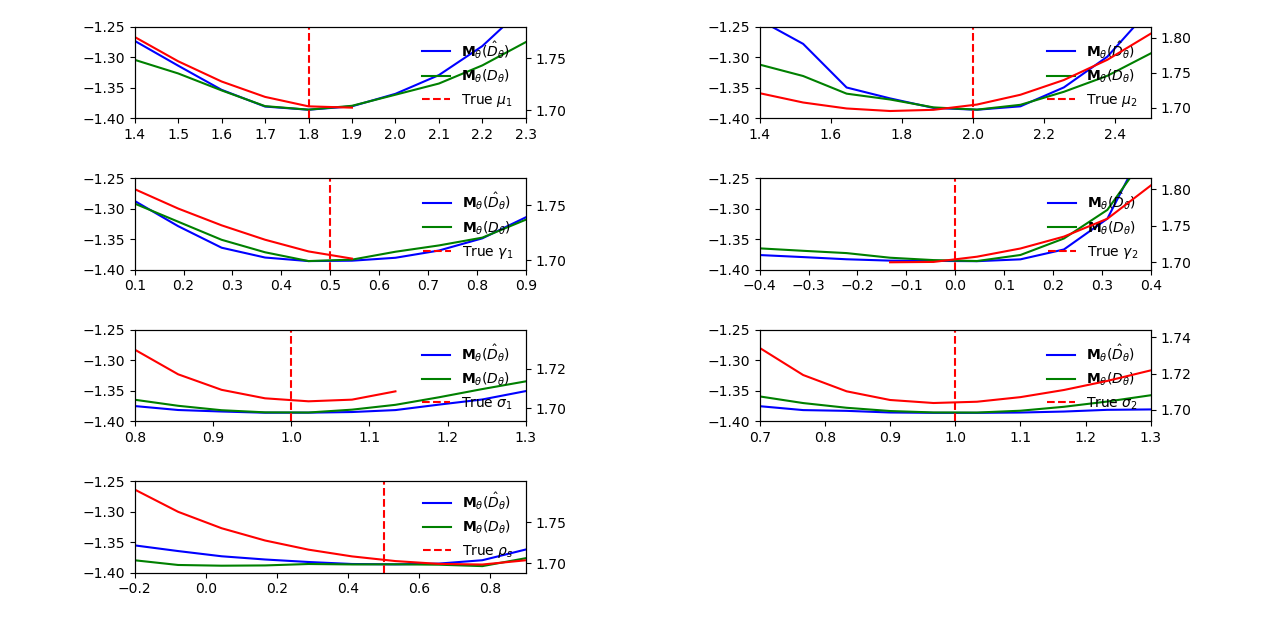
\includegraphics[width=\textwidth]{./Images/kmp_figure_6.png}
    \caption{Replication of Figure 6 in \cite{kaji2023adversarial}}
    \label{fig:kmp_figure_6}
\end{figure}

\begin{figure}
    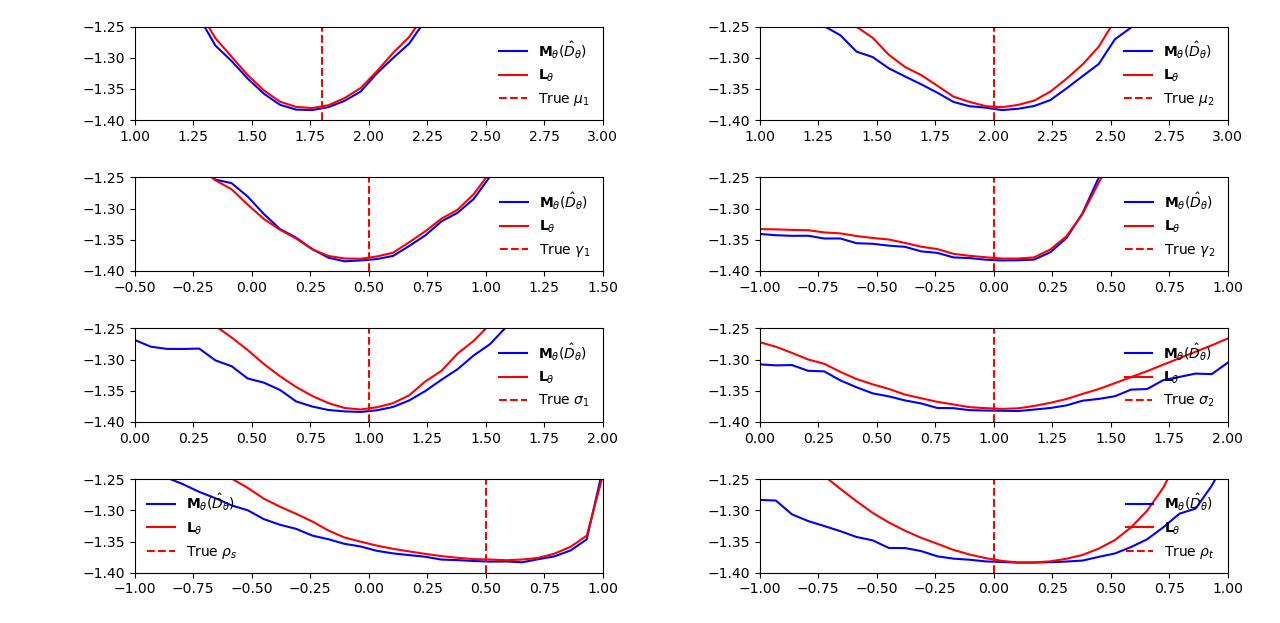
\includegraphics[width=\textwidth]{./Images/kmp_figure_8_sp.png}
    \caption{Replication of Figure 8 in \cite{kaji2023adversarial}}
    \label{fig:kmp_figure_8_sp}
\end{figure}

Figures \ref{fig:kmp_figure_6} and \ref{fig:kmp_figure_8_sp} match Figures 6 and 8 in \cite{kaji2023adversarial}, confirming that my replication in the scientific Python stack, including of the neural network discriminator is sufficiently close to the original.  

\begin{figure}
    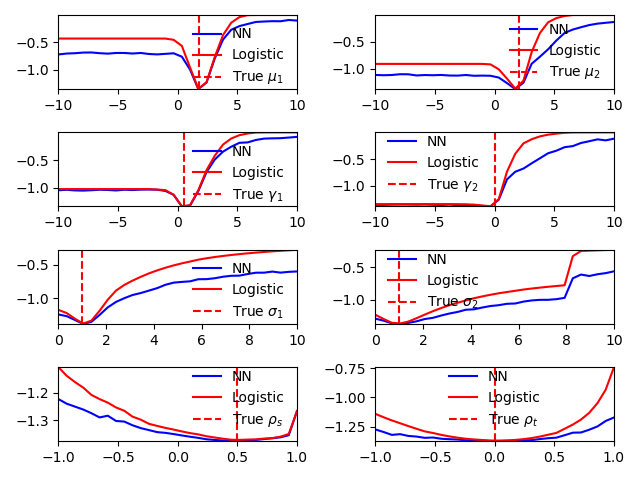
\includegraphics[width=\textwidth]{./Images/wide_loss_plots.png} %TODO verify how exactly this file was created!
    \caption{Losses cross-sections plotted over wider intervals}
    \label{fig:wide_loss_plots}
\end{figure}

Figure \ref{fig:wide_loss_plots} shows a variant of \ref{fig:kmp_figure_8_sp} plotted over wider intervals.
It is striking that for some parameters, the loss is flat when moving to far away from the optimal value.
Partly, this can be explained by the discrete choice nature of the Roy model.
Consider for example $\mu_1$.
If it becomes to small relative to $mu_2$ while $\gamma_1$ and $\gamma_2$ are held constant, the agents stop chosing sector 1.
Since only their chosen sectors and wages are observed, in such cases there are no observations that help to narrow down the vale of $\mu_1$ (except to bound it from above).
Similar arguments explain the flatness towards the tail of the cross-hairs for all four location parameters $\mu_1$, $\mu_2$, $\gamma_1$, and $\gamma_2$. %TODO verify

\begin{figure}
    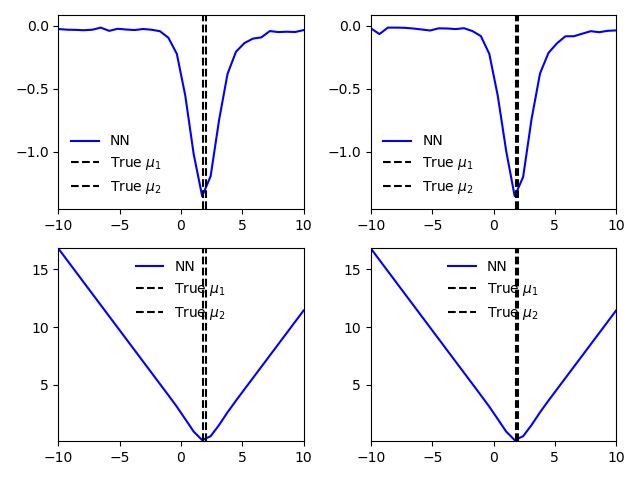
\includegraphics[width=\textwidth]{./Images/diagonal_loss_plots CE wasserstein-1.png} %TODO verify how exactly this file was created!
    \caption{Diagonal loss cross-sections. Rows: Jensen-Shannon divergence, Wasserstein-1. Columns: $(\mu_1, \mu_2)$, $(\mu_1, -\mu_2)$.}
    \label{fig:diagonal_loss_plots}
\end{figure}

Recall from section \ref{sec:ce_loss} that there is another reason for the loss-function to become flat,
at at least for the neural network estimator with cross-entropy loss.
Namely, the constant Jensen-Shannon divergence for disjoint distributions.
To isolate the effect, I rotate part of the cross-hairs to look at the loss along the diagonal $\{(\mu_1$, $\mu_2) = (m, m); m \in \mathbb{R}\}$.
This way, the fake distribution can become disjoint from the real distribution without affecting the agents' choices.
\footnote{There is a small distortion because $\mu_1 = 1.8 \neq 2.0 = \mu_2$.}

Figure \ref{fig:diagonal_loss_plots} shows the results:
In the top row, a neural network discriminator approximates the JS divergence.
The the bottom row, the Wasserstein-1 distance as approximated by the Sinkhorn divergence is plotted.
The left column shows clearly that the Jensen-Shannon divergence becomes constant when ($\mu_1$, $\mu_2$) is small or big enough that the distributions become disjoint, while the Wasserstein-1 distance provides constant gradients.
The right column plots the diagonal $\{(\mu_1$, $-\mu_2) = (m, m); m \in \mathbb{R}\}$: disjointness is also realized in this case for large absolute values of ($\mu_1$, $\mu_2$).

\subsection{Estimation}

\begin{figure}
    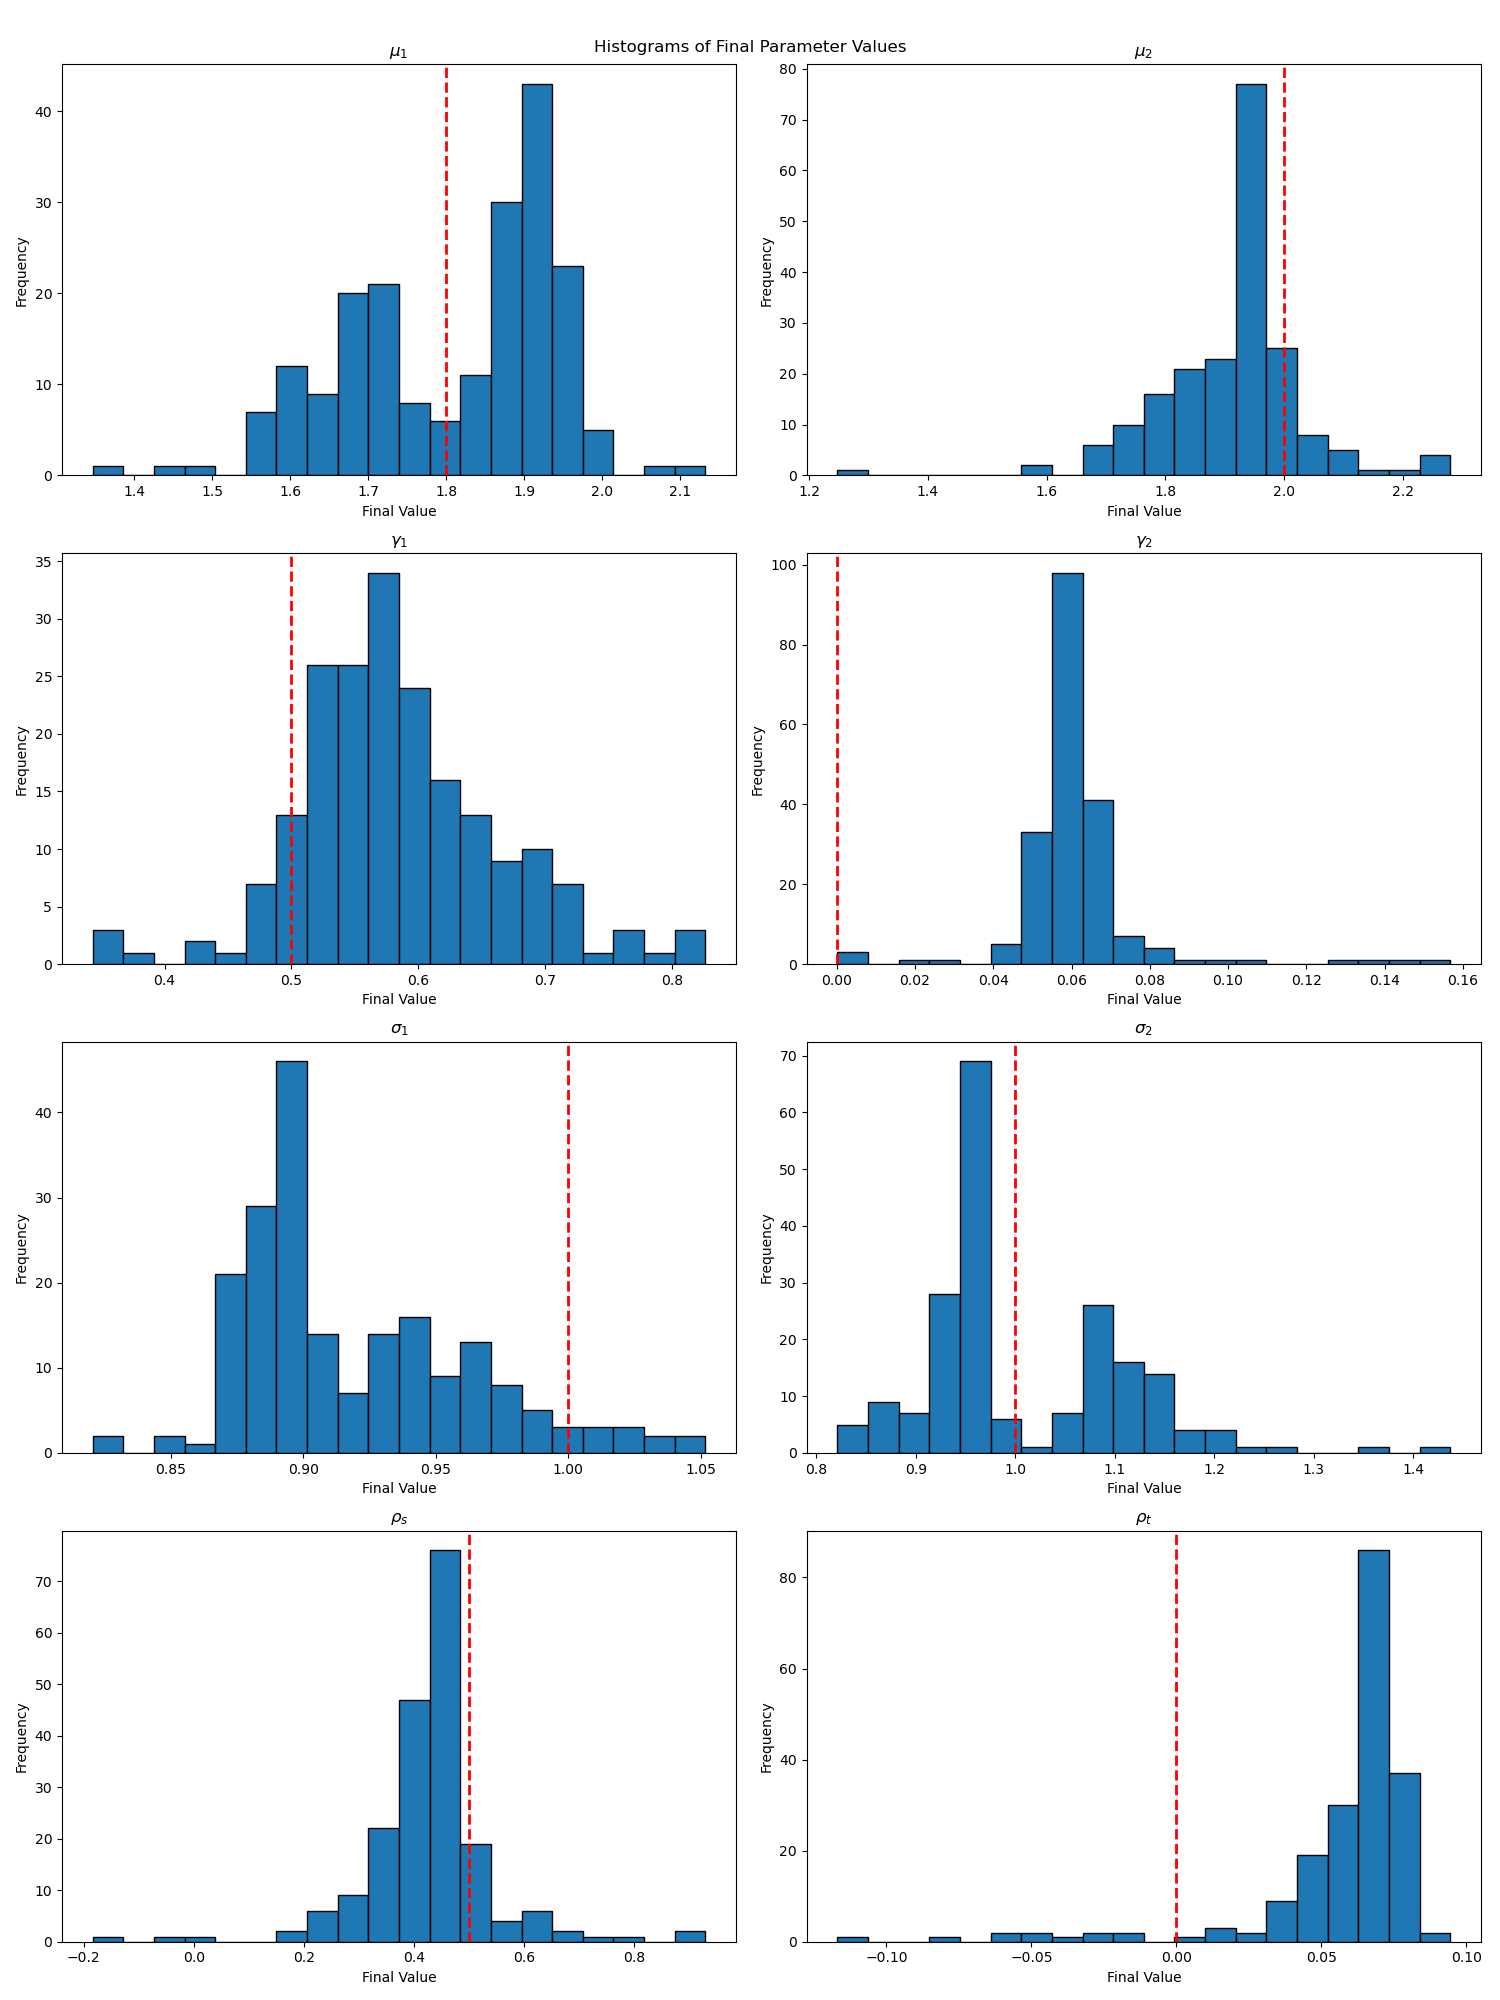
\includegraphics[width=\textwidth]{./Images/main_case_histograms.png}
    \caption{Results of 200 bootstrap estimations with Wasserstein-1 loss}
    \label{fig:main_case_histrograms}
\end{figure}

\begin{table}
    \centering
    \begin{tabular}{|l|c|c|c|c|c|c|c|c|}
    \hline
    & $\mu_1$ & $\mu_2$ & $\gamma_1$ & $\gamma_2$ & $\sigma_1$ & $\sigma_2$ & $\rho_s$ & $\rho_t$ \\
    \hline
    Wasserstein-1-discriminator & 1.81 & 1.91 & 0.58 & 0.06 & 0.92 & 1.01 & 0.43 & 0.06 \\
    & (0.14) & (0.12) & (0.08) & (0.02) & (0.04) & (0.10) & (0.12) & (0.03) \\
    \hline
    Wasserstein-1-discriminator with uniform initialization on wide intervals & -0.97 & -0.74 & -1.31 & -2.36 & 1.78 & 2.05 & -0.10 & -0.05 \\
    & (4.48) & (4.19) & (4.72) & (4.95) & (1.88) & (1.99) & (0.67) & (0.53) \\
    \hline
    \end{tabular}
    \caption{Parameter estimates}
    \label{tab:parameter_estimates}
\end{table}

I reproduce the simulations in section 3.2.2 of \textcite{kaji2023adversarial} using the approximate Wasserstein-1 estimator implemented in \texttt{geomloss.SamplesLoss} and 200 bottstrap samples.
The first row of \ref{tab:parameter_estimates} shows the results.
% mu_1 closer mu_2 closer gamma_1 closer gamma_2 as close as worst, sigma_1 as close as worst sigma_2 closer rho_s as close as worst rho_t middle
The point estmimates are always at least as close to the true parameter values as those reported in Table I of \cite{kaji2023adversarial}.
The standard errors are also comparable or tighter except for $\mu_1$ and $\mu_2$.

Figure \ref{fig:main_case_histrograms} visualizes the distribution of estimates.

\begin{figure}
    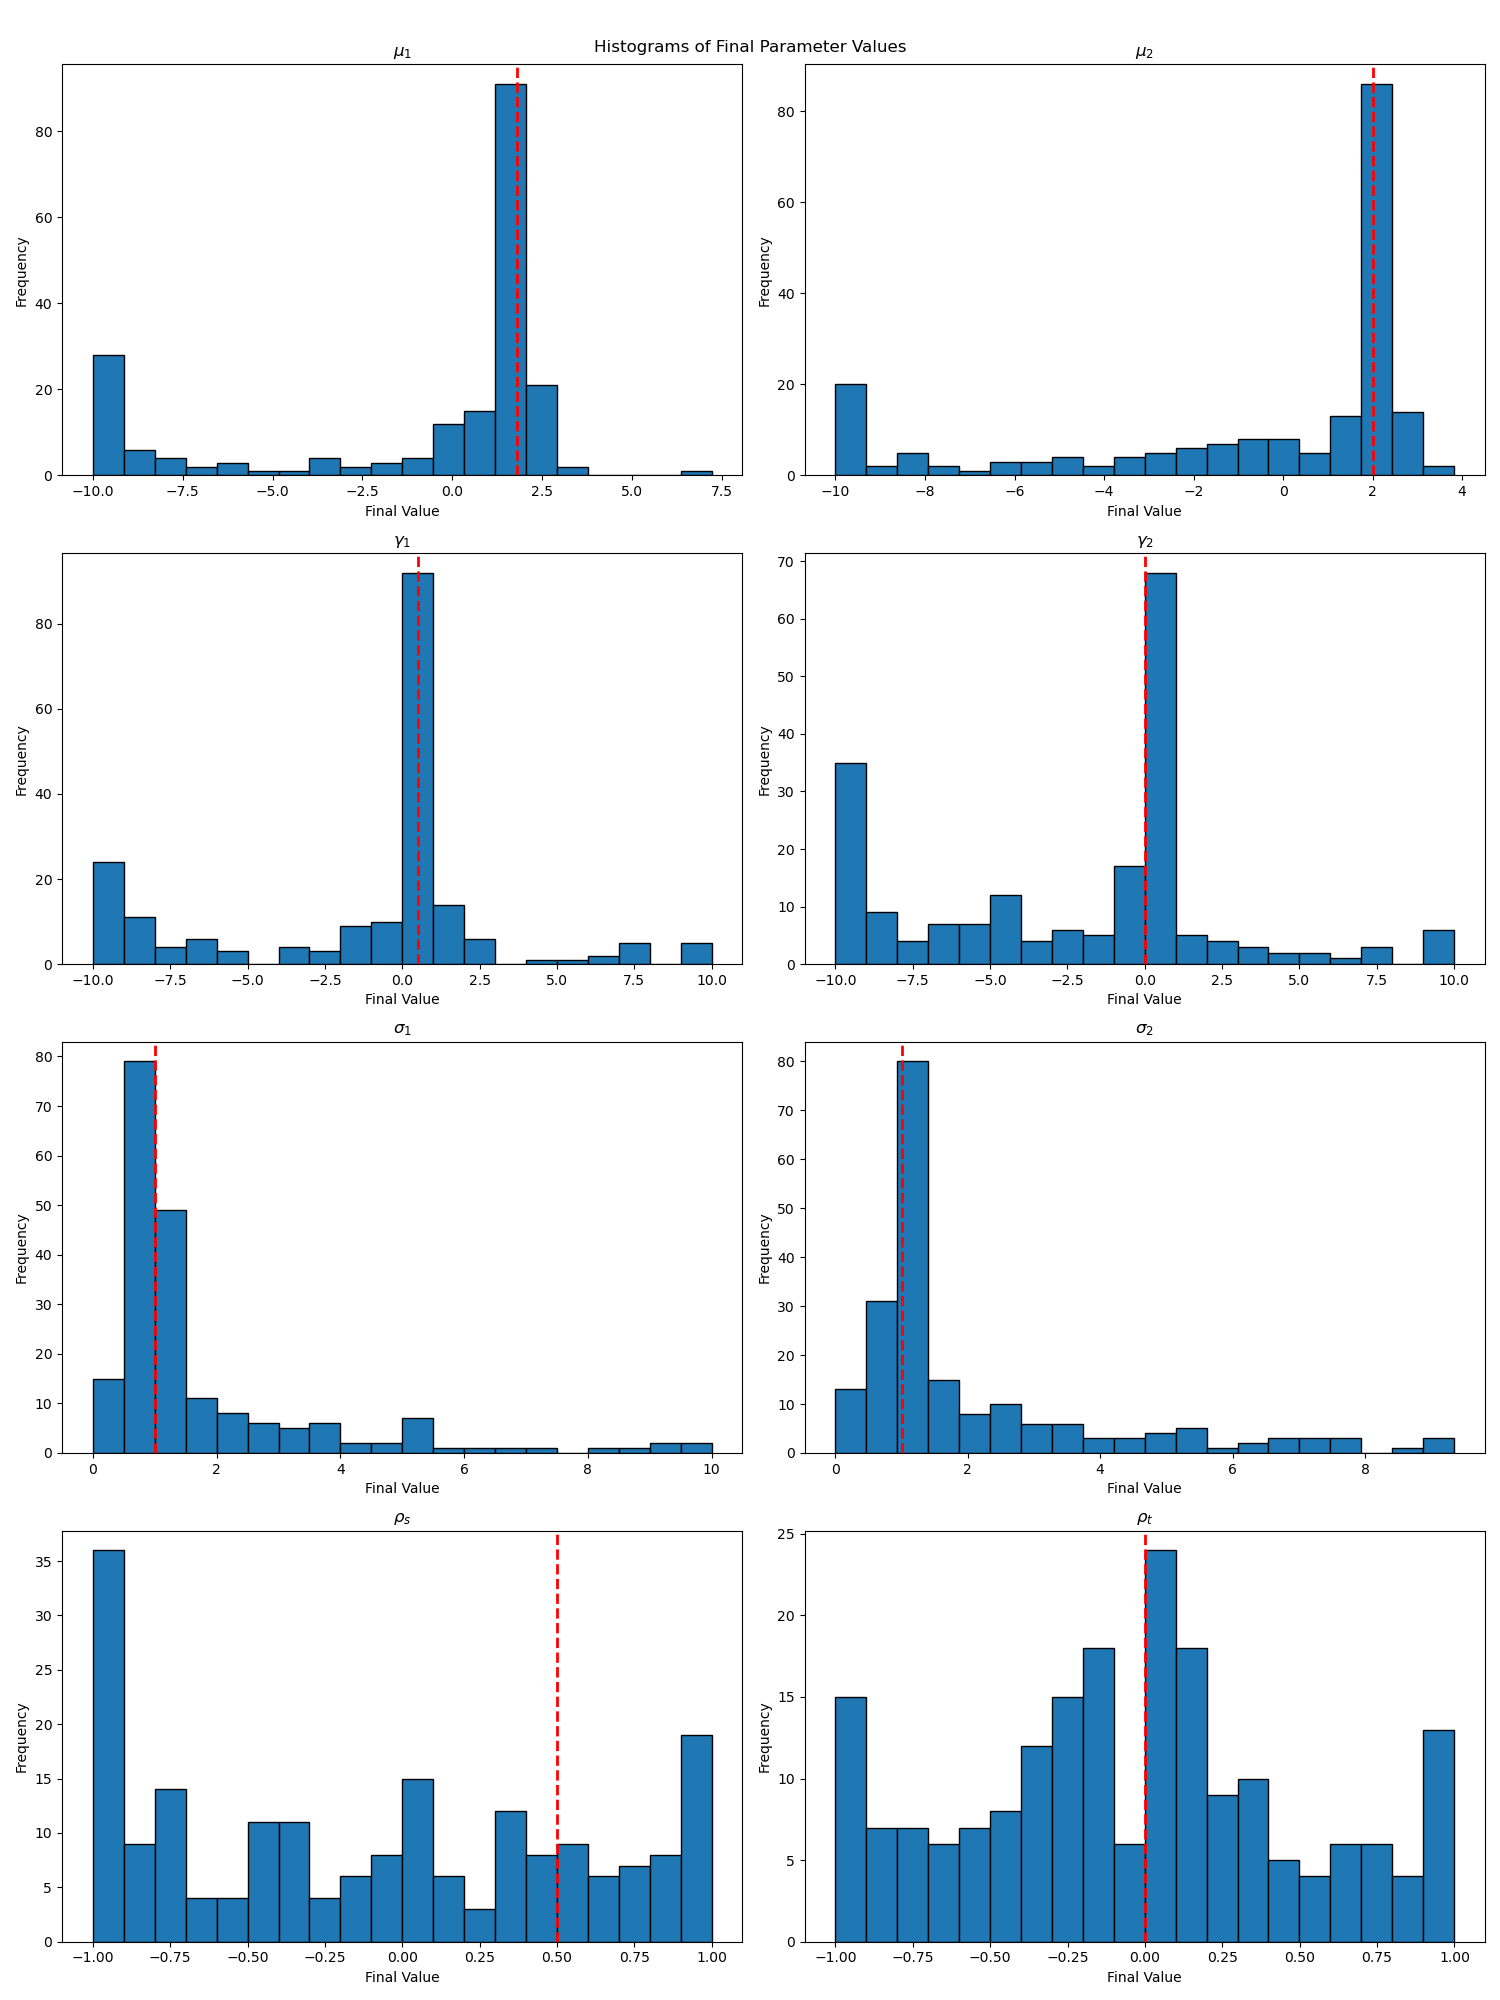
\includegraphics[width=\textwidth]{./Images/wide_uniform_histograms.png}
    \caption{Results of 200 estimations with Wasserstein-1 loss and initial values that are uniform over broad intervals}
    \label{fig:wide_uniform_histograms}
\end{figure}

